\subsubsection{Field Cage for protoDUNE Dual Phase}
Field cages provide uniform electric fields for ionization electrons to drift to anodes for the detection in the Time Projection Chamber.
The baseline design for DUNE LAr TPC is that of the single phase in which the ionization electrons created by the secondary particles 
resulting in neutrino-nucleon interactions drift in LAr and get detected on the anode plane that resides inside the liquid phase of argon.  An alternative technology is the LAr TPC that the ionization electrons drift through LAr but then extracted through the strong extraction field at the top of the liquid and detected in the anode in gaseous phase of argon after a signal amplification via an large area gas electron multiplier (LEM), hence the dual phase.

During the period of his sabbatical stay at CERN, Yu has begun to work on WA105, a dual phase $6m\times 6m\times 6m$ prototype testing project at CERN through the participation in the smaller prototype cosmic ray detector in $1m\times 1m\times 3m$.  This work provided an opportunity for UTA IF group to join WA105 as the first U.S. group and to position itself well to play a leading role in dual phase.   While dual phase technology is currently at a lower priority to the single phase LAr TPC, it is clear that U.S. groups' participation in alternate technology is beneficial in many perspectives, including that of strengthening the international nature of DUNE collaboration an essential ingredient in its success.

As the schedule for DUNE experiment and for the two protoDUNE experiments get clearer, it became apparent that UTA will be able to play an importnat role in design and construction of these experiments.   The overarching strategy in identifying the construction was to ensure UTA's contribution to any of the two protoDUNE experiment would aim to direct participation in DUNE from the first 10kt module in early 2020s.  One such component easily identifiable is the field cage for which the collaboration is targetting to utilize as much common components as possible for single phase and dual phase protoDUNE detectors.    With this premise, Yu has discussed with the DUNE management and has agreed to take the responsibility in design and construciton of dual phase field cage together with the University of Zurich group.    

Figure~\ref{fig:if-dp-fc} shows the current conceptual design of the field cage for the dual phase protoDUNE experiment.   The primay concept of this field cage is to use compartmentalized structure of submodules that consist of several straight profiles to provide voltage differentials for the generation of uniform fields.   The use of straight profiles made of either aluminium or stanless steel makes the preassembly and shipment of submodules convenient.   Each of these submodules will be prepared to the quality to hold high voltages at 180kV (for single phase) or  360kV (for dual phase) over the drift length.  
\begin{figure}[htb]
\centering
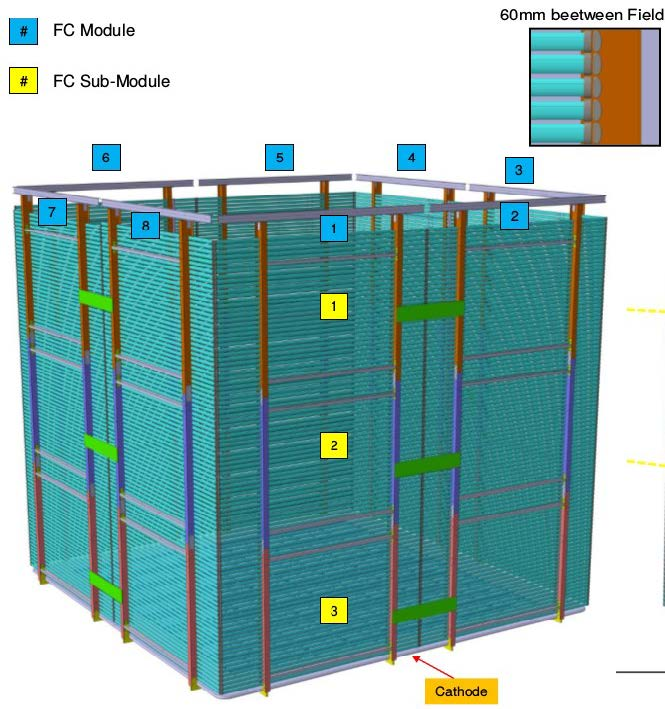
\includegraphics[width=0.80\textwidth]{images/if-dp-fc.jpg}
\caption[]{Conceptual skematic drwaing of the field cage assembly for dual phase protoDUNE.}
\label{fig:if-dp-fc}
\end{figure}

At present, it has been agreed that either CERN or Fermilab will be responsible for purchasing and production of the necessary mechanical parts, including the I--beams that act as the spine of the submodule and the each profile.  The project funds will pay for the purchase electrical parts - voltage divider resisters and varisters for surge arresting - and the production of electronic boards the field cage.  UTA will work with the single phase field cage group, including BNL team, and the single phase field cage electronics group at Louisiana State University as well as the University of Zurich group on design of both the mechnical and electrical part of the dual phase field cage.   We will be responsible for preassembly of the field cage submodules, mouting of the electric boards, testing of each submodules and performaning functional prototype testing with as large a field cage as possible before shipping the dissembled submodules out to CERN for installation.

For the completion of the design of the dual phase field cage, our postdoctoral fellow, Animesh Chatterjee will be stationed at CERN starting from October 2016 through mid January 2017.   During this period, Chatterjee will work with the ETH and CERN groups to  
